\documentclass[a4paper, 14pt]{article}
\usepackage[utf8]{inputenc}
\usepackage{amsmath,amsfonts,amssymb,amsthm,mathtools} % AMS
\usepackage{wrapfig,lipsum,cleveref}
\usepackage{icomma} 
\usepackage{listings}
\usepackage{color}
\usepackage{geometry} 
\usepackage{longtable}

\linespread{1.5}

\geometry{top=25mm}
\geometry{bottom=35mm}
\geometry{left=35mm}
\geometry{right=20mm}

\definecolor{codegreen}{rgb}{0,0.6,0}
\definecolor{codegray}{rgb}{0.5,0.5,0.5}
\definecolor{codepurple}{rgb}{0.58,0,0.82}
\definecolor{backcolour}{rgb}{0.95,0.95,0.92}
\definecolor{codered}{rgb}{0.130,0,0}
\definecolor{codedodgerblue}{rgb}{0.176,0.224,0.230}
\lstdefinestyle{mystyle}{
	backgroundcolor=\color{backcolour},   
	commentstyle=\color{codedodgerblue},
	keywordstyle=\color{codegreen},
	numberstyle=\tiny\color{codegreen},
	stringstyle=\color{codered},
	basicstyle=\footnotesize,
	breakatwhitespace=false,         
	breaklines=true,                 
	captionpos=b,                    
	keepspaces=true,                 
	numbers=left,                    
	numbersep=5pt,                  
	showspaces=false,                
	showstringspaces=false,
	showtabs=false,                  
	tabsize=2
}
\lstset{style=mystyle}

%% Номера формул
\mathtoolsset{showonlyrefs=true} % Показывать номера только у тех формул, на которые есть \eqref{} в тексте.

%% Шрифты
\usepackage{euscript}	 % Шрифт Евклид
\usepackage{mathrsfs} % Красивый матшрифт

%% Свои команды
\DeclareMathOperator{\sgn}{\mathop{sgn}}

%% Перенос знаков в формулах (по Львовскому)
\newcommand*{\hm}[1]{#1\nobreak\discretionary{}
{\hbox{$\mathsurround=0pt #1$}}{}}


\title{Вариация алгоритма кросс-валидации со взвешиванием наблюдений}
\usepackage{cmap}					% поиск в PDF
\usepackage[T2A]{fontenc}			% кодировка
\usepackage[utf8]{inputenc}			% кодировка исходного текста
\usepackage[english,russian]{babel}	% локализация и переносы
\usepackage{graphicx}
\graphicspath{{pictures/}}
\DeclareGraphicsExtensions{.pdf,.png,.jpg}
\author{Гармидер Петр}
\date{\today}
\begin{document}


\thispagestyle{empty}
\begin{center}
	\textbf{ПРАВИТЕЛЬСТВО РОССИЙСКОЙ ФЕДЕРАЦИИ}\\
	\vspace{2ex}
	\textbf{Федеральное государственное автономное\\ образовательное учреждение высшего образования}
	
	\vspace{2ex}
	
	\textbf{Национальный исследовательский университет \\ <<Высшая школа экономики>>}
	
	\vspace{8ex}
	\begin{flushright}
		Факультет экономических наук\\
		Образовательная программа <<Экономика>>
	\end{flushright}
\end{center}
\vspace{9ex}

\begin{center}
	{\textbf{КУРСОВАЯ РАБОТА
	}}
	\vspace{1ex}
	
	На тему <<Вариация алгоритма кросс-валидации со взвешиванием наблюдений>>
\end{center}
\vspace{1ex}
\begin{flushright}
	\noindent
	Студент группы БЭК161\\Гармидер Петр Александрович\\
	\vspace{13ex}
	Научный руководитель:\\
	Борис Демешев
	
\end{flushright}	

\vfill

\begin{center}
	Москва 2019
	
\end{center}
\newpage

\tableofcontents

\newpage

\section{Введение}
\subsection{Параметры и гиперпараметры модели}
Большая часть популярных моделей имеют множество параметров и гиперпараметров однозначно выделяющие модель из множества всех алгоритмов. Гиперпараметры модели --- параметры, вводимые пользователем вручную, которые в большинстве случаев не меняются в ходе обучения\footnote{Однако такая практика также используется, например, изменение гиперпараметра  learning rate в ходе алгоритма градиентного спуска (см. \cite{zeiler2012adadelta})}. Параметры модели --- параметры, которые не вводятся пользователем вручную, а есть результат оптимизации функции потерь. Их конечное значения становится известно после завершения процесса обучения. Параметры модели связывают имеющиеся у исследователя данные и выбранный алгоритм для обучения. 

Рассмотрим пример. Пусть имеем обучающую выборку $D = \left\{x_i, y_i\right\}$ и тестовую выборку $d = \left\{x_i, y_i\right\}$, где $x_i$, $y_i$ $\in R$, $\left|D\right| = N$ и $\left|d\right| = n$. Будем оценивать $y_i$ используя $L_2$ - регуляризатор или Ridge-regression (см. \cite{hoerl1970ridge}). Имеем безусловной задачу оптимизации:


\begin{equation} 
\label{ridge} %% Invalid referencing
\sum_{i=1}^{N} (y_i - \hat{\beta_0} - \hat{\beta_1} x_i)^2 + \lambda \hat{\beta_1^2} \rightarrow min_{\hat{\beta_0}, \hat{\beta_1}}
\end{equation} 

В (\ref{eq: 1}) существуют два параметра для оптимизации $\hat{\beta_0} \text{ и } \hat{\beta_1}$, а также один гиперпараметр $\lambda$, который является константой в рассматриваемой задаче. Коэффициенты регрессии находятся из задачи минимизации при заданном уровне $\lambda$, в то время, как степень регуляризации $\lambda$ задается исследователем. В конечно счете исследователь заинтересован в создании модели, которая имеет высокое качество на тестовой выборке $d$, что не участвовала в процессе обучения. Качество работы модели на выборке $d$ очевидно зависит от выбранного исследователем $\lambda$. Поэтому, выбор оптимального значения для гиперпараметров является также важной задачи для получения лучшей модели.

Гиперпараметрами модели также могут быть: метод обработки пропусков в данных, количество слоев в нейронной сети, выбранные функции активации, уровень Dropout, скорость обучения и другие. 

Влияние гиперпараметров на качество работы модели делает их правильный выбор отдельной задачей. Оптимальный алгоритм подбора гиперпараметров уникален для каждой конкретной задачи. Качество работы модели в целом принято оценивать на выборках не участвовавших в обучении, но для которых известно истинной значение зависимой переменной. 

\subsection{Типы кросс-валидации}
Кросс-валидация --- техника валидации модели для оценки качества её работы и установления факта обобщающей способности. Метод CV позволяет понять, выучила ли модель зависимость между рассматриваемыми переменными или же алгоритм переобучился и хорошо предсказывает лишь данные имеющиеся в обучающей выборке\footnote{В английской литературе данную ситуацию называют 	overfitting}. Как правило, кросс-валидационной проверке подвергаются модели, которые направлены на точность предсказаний, оставляя за бортом вопрос интерпретации полученных результатов.  

\noindent Разберем некоторые варианты алгоритма кросс-валидации:

\noindent Пусть имеем: $X$ --- множество признаков, описывающих объекты; $Y$ --- множество зависимых переменных; $D^l = \left\{x_i, y_i\right\}$ --- наблюдаемая выборка , где $x_i \in X$, $y_i \in Y$, $l$ --- размер выборки; $Q : (A \times (X \times Y ) )  \rightarrow R$ --- функция потерь; $A$ --- модель; $\mu : (X \times Y) \rightarrow A$ --- алгоритм обучения \cite{ifmocv}.

\label{CV_methods}
\begin{itemize}
	\item Валидация на отложенных данных (Hold-out)
	
	Исследователь выбирает число $t$ --- количество объектов из множества $D$, которые будут использованы для обучения модели. Соответственно, оставшая часть объектов $l - t$ используется для проверки качетсва работы модели. Итого, получаются две выборки $Train^t \text{ и } Test^{l-t}$ такие, что $Tr^t \cup Tt^{l-t} = D^l$. Решается задача:
	
	\[HOCV(\mu, Tr^t, Tt^{l-t}) = Q(\mu (Tr^t), Tt^{l-t}) \rightarrow min_{\mu} \] 
	
	\begin{figure}[h]
		\center{
\includegraphics[scale=0.55]{img/Hold-out}}
		\label{ris: ho}
		\caption{Иллюстрация валидации на отложенных данных}
	\end{figure}
	
	
	Метод Hold-out CV обычно используется в том случае, если исследователь обладает большой обучающей выборкой, т.к данный способ не требует больших вычислительных мощностей. Итоговое качество $Q$ также зависит от разбиения обучающей выборки, что является главным недостатком метода. 
	
	\item K-fold кросс-валидация 
	
	Исходная выборка $D$ разбивается случайным образом на $K$ непересекающихся, примерно равных по мощности множеств: $D_1$, $D_2$, $\dots$ $D_k$; $\left|D_i\right| \approx \frac{l}{k}$. После чего, для каждого из получившихся множеств проводится процедура hold-out CV; результаты всех процедур усредняются. Решается задача:
	
	\[KFCV(\mu, D, K) = \frac{1}{K} \sum_{i=1}^{K} OFCV(\mu(D \textbackslash D_i), D_i) \rightarrow min_{\mu} \]
	
	\begin{figure}[h]
		\center{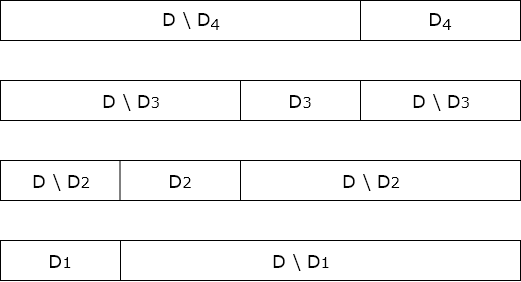
\includegraphics[scale=0.55]{img/K_CV}}
		\label{ris: kfold}
		\caption{Иллюстрация K-fold кросс-валидации при K = 4}
	\end{figure}
	
	Метод K-fold CV решает проблему высокой зависимости получаемого результата от разбиения, однако является весьма затратным с точки зрения вычислительных мощностей. Обычно используется в тех случаях, когда размеры выборки и модель позволяют быстро проводить процедуру обучения. Число K выбирается исследователем на своё усмотрение. Заметим, что при $t = \frac{l}{2}$ Hold-out CV $ \equiv $ two-fold CV.
	
	\item Leave-one-out кросс-валидация
	
	Частный случай K-fold кросс-валидации, при $K=l$. Исходное множество $D$ разбивается на $l$ подмножеств: $D_1$, $D_2$, $\dots$ $D_l$; $\left|D_i\right| = 1$. После чего проводится стандартная K-fold кросс-валидация. LOO CV подвергается критике; в некоторых исследованиях говорится, что данный метод плохо оценивает предсказательную силу модели \cite{efron1986biased}. Кроме того, данный метод требует высоких вычислительных мощностей, т.к потребуется $l$ раз обучать модель.
	
	\item Полная кросс-валидация (Complete)
	
	Исследователь выбирает число $t$, после чего изначальная выборка $D^l$ разбивается всеми возможными способами на выборки $Tr^l$ и $Tt^{l-t}$. Заметим, что силов возможных разбиений для заданного t равно $C_l^{l-t}$. Таким образом, исследователь решает задачу:
	
	\[CCV(D, t) = \frac{1}{C_l^{l-t}} \sum_{D^l = Tr^l \cup Tt^{l-t}} Q(\mu (Tr^t), Tt^{l-t}) \rightarrow min_{\mu} \]
	
	Даже при достаточно небольших значениях t, данный метод проверки работоспособности модели используется крайне редко в силу его вычислительной сложности.
	
	\item Случайные разбиения (Random sampling)
	
	Выборка разбивается в случайной пропорции, после чего для получившегося разбиения проводится hold-out CV. Данная процедура повторяется несколько раз; результаты усредняются. 
	
	
	\item M $\times$ K-fold кросс-валидация
	
	K-fold кросс-валидация проводится M раз; результаты М валидаций усредняются. Итого: 
	
	\[MKFCV(\mu, D, K, M) = \frac{1}{M} \sum_{i=1}^{M} KFCV(\mu, D, K) \rightarrow min_{\mu}  \]
	
	Метод допустим к использованию при небольшой выборке и алгоритме, который способен обучаться $M \times K$ раз за разумное время.
\end{itemize}
\label{fkdsfsdfdsa}

Одной из причин использования кросс-валидации является подбор гиперпараметров. Допустим исследователь решает задачу по выбору оптимального параметра $\lambda$ для $L_2$ - регуляризатора на странице \pageref{ridge}. Если не проводить кросс-валидацию, то лучшее качество на выборке $D$ даст модель с $\lambda = 0$, т.к в этом случае на коэффициенты регрессии не накладываются никакие ограничения, а поэтому они сойдутся к решению, которое минимизирует среднеквадратичную ошибку на выборке $D$. Однако, получаемое качество работы модели на обучающей выборке не отображает реальную картину. Исследователь, в конечном счете, заинтересован создать модель, которая будет иметь высокое качество на объектах не входящих в обучающую выборку. Для этого, есть смысл проверять качество работы модели используя один из перечисленных методов кросс-валидации. В этом случае, оптимальное значение $\lambda$ скорее всего окажется больше нуля.

\subsection{Кросс-валидация на временных рядах}

Временной ряд --- наблюдаемая выборка данных, объекты которой представлены во временном порядке. В большинстве случаев, временной ряд представлен точками, которые одинаково отдалены друг от друга во временной шкале. Анализ временных рядов значимо отличается от подходов работы с простой выборкой данных:  учитывается зависимость точек от времени, а также взаимосвязь текущего значения параметра с лагированными. Примерами временных рядов являются: курс доллар к евро, реальный уровень ВВП США, ключевая ставка ЦБ РФ, последовательность кадров в видеоролике и так далее. В данной работе фокус будет сделан на одномерных временных рядах, прогноз для которых будет иметь вид некоторой функции от прошлых значений. 

Как и раньше, задача построения моделей для прогнозирования временных рядов включает в себя стадию подбора оптимальных гиперпараметров модели. Однако, по очевидным причинам большинство методов кросс-валидации из секции \ref{CV_methods} не подходят для случая, когда объектом исследования является временной ряд. Непрактично оценивать модель на случайно выбранных данных, которые с большой долей вероятности потеряют временную структуру при разбиениях. 



\newpage
\bibliographystyle{utf8gost705u}  %% стилевой файл для оформления по ГОСТу
\bibliography{biblio}     %% имя библиографической базы (bib-файла) 


\end{document}
